%!TEX root = presentazionelancia.tex
\section{Architecture}
\begin{frame}[t]
\frametitle{Architecture}
    \onslide<1>Before Tao
    \begin{center}
    	\includegraphics<1>[width=0.6\textwidth]{figs/before_tao.jpg}
    \end{center}
	\onslide<2>After Tao
	\begin{center}
    	\includegraphics<2>[width=0.6\textwidth]{figs/tao_arch.jpeg}
    \end{center}
\end{frame}

\begin{frame}[fragile]
\frametitle{Storage Layer}
\begin{itemize}
	\item Object and Associations are stored in MySql (before \& with TAO)	
	\item TAO API is mapped to a small set of SQL queries
	\item A single MySql server can't handle TAO volumes of data
	\begin{itemize}
		\item We divide data into logical \emph{shards}
		\item \emph{shards} are mapped to db 
		\item different servers are responsible for multiple shards
		\item mapping is adjusted for load balancing
	\end{itemize}
	\item Object are bounded to a \emph{shard} for their entire lifetime
	\item Associations are stored in the \emph{shard} of its \verb!id1!
\end{itemize}
\end{frame}

\begin{frame}[c]\frametitle{Cache Layer}
    TAO cache 
    \begin{itemize}
    	\item contains: Objects, Associations, Associations counts
    	\item implement the complete API for clients
    	\item handles all the communication with storage layer
    	\item it's filled on demand end evict the least recently used items
    	\item Understand the semantic of their contents
    \end{itemize}

    It consists of multiple servers forming a \emph{tier}
    \begin{itemize}
    	\item Request are forwarded to correct server by a \emph{sharding} scheme as dbs
    	\item For cache miss and write request, the server contacts other caches or db
    \end{itemize}
    
\end{frame}
\begin{frame}[c]\frametitle{Yet Another caching layer}
	\onslide<1->\textbf{Problem: }A single caching layer divided into a \emph{tier} is susceptible to \emph{hot spot}

	\onslide<2->\textbf{Solution: }Split the caching layer in two levels
	\onslide<2->\begin{itemize}
		\item A \emph{Leader} tier
		\item Multiple \emph{Followers}	tiers
	\end{itemize}
\end{frame}

\begin{frame}[c]\frametitle{Leaders \& Followers}
   	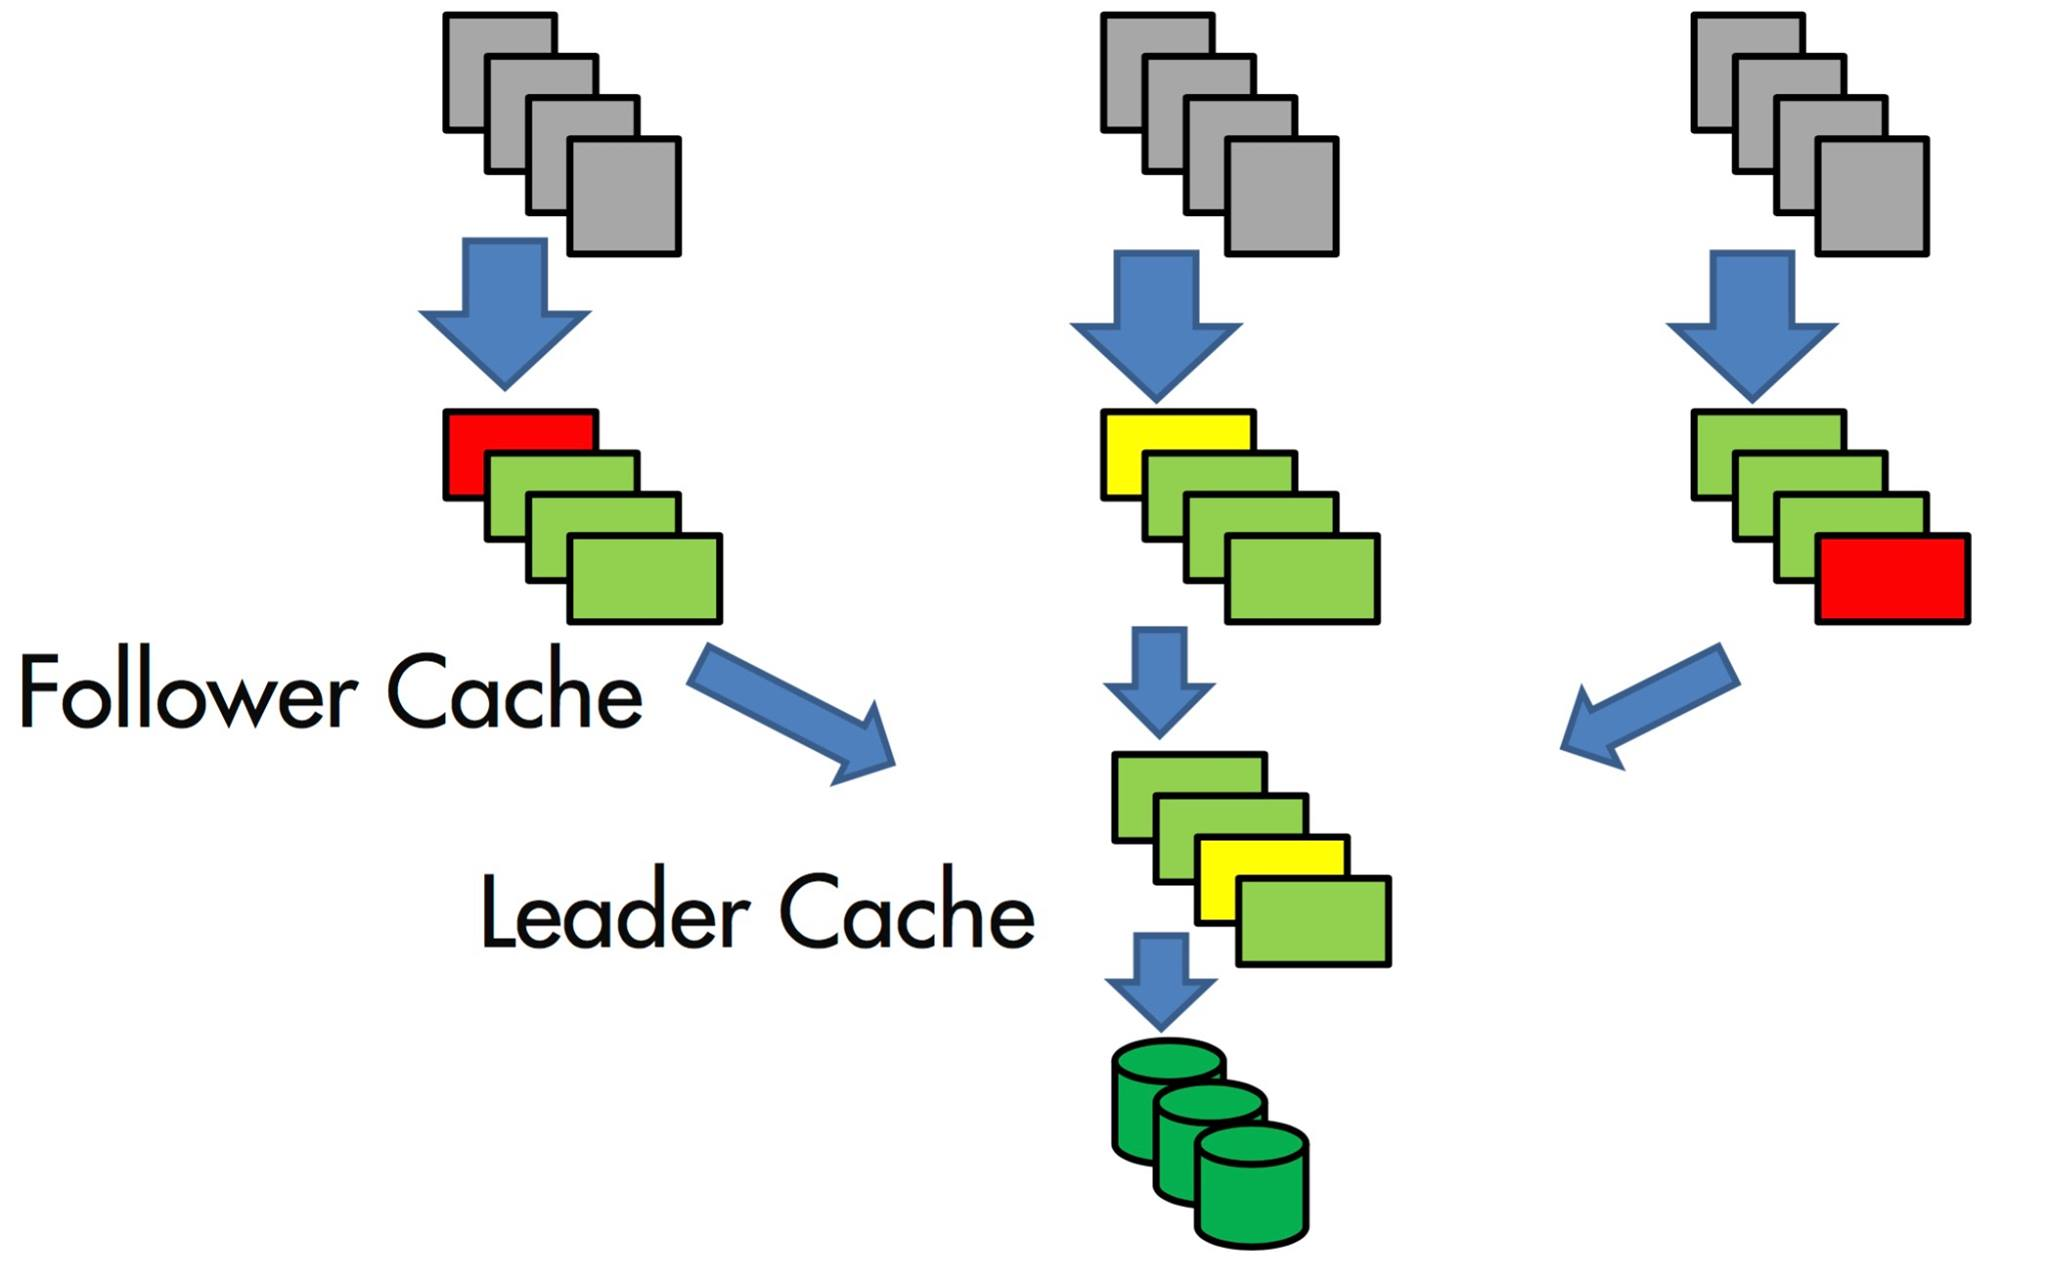
\includegraphics[width=\textwidth]{figs/followers_leader.jpeg}
\end{frame}

\begin{frame}[c]\frametitle{Leaders \& Followers}
    \begin{itemize}
    	\item Followers forward all writes and read cache misses to the leader tier
		\item Leader sends async cache maintenance messages to follower tier
		\begin{itemize}
			\item Eventually Consistent
		\end{itemize}
		\item If a follower issues a write, the follower’s cache is updated synchronously
		\item Each update message has a version number
		\item Leader serializes writes
    \end{itemize}


\end{frame}

